% \documentclass[handout]{beamer}
\documentclass{beamer}

\mode<presentation>
{
  \usetheme{ANLBlue}
  % \usefonttheme[onlymath]{serif}
  % \usetheme{Singapore}
  % \usetheme{Warsaw}
  % \usetheme{Malmoe}
  % \useinnertheme{circles}
  % \useoutertheme{infolines}
  % \useinnertheme{rounded}

  \setbeamercovered{transparent=20}
}

\usepackage[english]{babel}
\usepackage[latin1]{inputenc}
\usepackage{alltt,listings,multirow,ulem,siunitx}
\usepackage[absolute,overlay]{textpos}
\TPGrid{1}{1}
\usepackage{pdfpages}
\usepackage{ulem}
\usepackage{multimedia}
\usepackage{multicol}
\newcommand\hmmax{0}
\newcommand\bmmax{0}
\usepackage{bm}
\usepackage{comment}
\usepackage{subcaption}

% font definitions, try \usepackage{ae} instead of the following
% three lines if you don't like this look
\usepackage{mathptmx}
\usepackage[scaled=.90]{helvet}
% \usepackage{courier}
\usepackage[T1]{fontenc}
\usepackage{tikz}
\usetikzlibrary{decorations.pathreplacing}
\usetikzlibrary{shadows,arrows,shapes.misc,shapes.arrows,shapes.multipart,arrows,decorations.pathmorphing,backgrounds,positioning,fit,petri,calc,shadows,chains,matrix}

\newcommand\vvec{\bm v}
\newcommand\bvec{\bm b}
\newcommand\bxk{\bvec_0 \times \kappa_0 \cdot \nabla}
\newcommand\delp{\nabla_\perp}

% \usepackage{pgfpages}
% \pgfpagesuselayout{4 on 1}[a4paper,landscape,border shrink=5mm]

\usepackage{JedMacros}

\newcommand{\timeR}{t_{\mathrm{R}}}
\newcommand{\timeW}{t_{\mathrm{W}}}
\newcommand{\mglevel}{\ensuremath{\ell}}
\newcommand{\mglevelcp}{\ensuremath{\mglevel_{\mathrm{cp}}}}
\newcommand{\mglevelcoarse}{\ensuremath{\mglevel_{\mathrm{coarse}}}}
\newcommand{\mglevelfine}{\ensuremath{\mglevel_{\mathrm{fine}}}}

%solution and residual
\newcommand{\vx}{\ensuremath{x}}
\newcommand{\vc}{\ensuremath{\hat{x}}}
\newcommand{\vr}{\ensuremath{r}}
\newcommand{\vb}{\ensuremath{b}}

%operators
\newcommand{\vA}{\ensuremath{A}}
\newcommand{\vP}{\ensuremath{I_H^h}}
\newcommand{\vS}{\ensuremath{S}}
\newcommand{\vR}{\ensuremath{I_h^H}}
\newcommand{\vI}{\ensuremath{\hat I_h^H}}
\newcommand{\vV}{\ensuremath{\mathbf{V}}}
\newcommand{\vF}{\ensuremath{F}}
\newcommand{\vtau}{\ensuremath{\mathbf{\tau}}}


\title{Exploits in Implicitness}
\subtitle{hardware, problem structure, and library design}
\begin{comment}
  Implicit solvers are uniquely powerful instruments for managing
disparate scales and performing analysis, but performance can be
subtle and challenging.  "Black-box" solvers suffer from limited
applicability and poor efficiency on modern hardware.  Building
efficient solvers relies increasingly on pairing problem-specific
structure with architectural capability and expressing the resulting
algorithms in terms of existing software.  Library design is the
inverse problem: create maximally-reusable components to satisfy a
diverse range of present and future customers and architectures.  This
talk discusses recent examples in PETSc's evolution and our vision for
implicit solvers.
\end{comment}

\author{{\bf Jed Brown} \texttt{jedbrown@mcs.anl.gov} (ANL and CU Boulder) \\
  Collaborators in this work: \\
  \quad Mark Adams (LBL), Peter Brune (ANL), Emil Constantinescu (ANL), \\
Debojyoti Ghosh (ANL), Matt Knepley (UChicago),  \\
Dave May (ETH Z\"urich, Lois Curfman McInnes (ANL), \\
Barry Smith (ANL))
}

% - Use the \inst command only if there are several affiliations.
% - Keep it simple, no one is interested in your street address.
% \institute
% {
%   Mathematics and Computer Science Division \\ Argonne National Laboratory
% }

\date{SIAM PP, 2014-02-21}

% This is only inserted into the PDF information catalog. Can be left
% out.
\subject{Talks}


% If you have a file called "university-logo-filename.xxx", where xxx
% is a graphic format that can be processed by latex or pdflatex,
% resp., then you can add a logo as follows:

% \pgfdeclareimage[height=0.5cm]{university-logo}{university-logo-filename}
% \logo{\pgfuseimage{university-logo}}



% Delete this, if you do not want the table of contents to pop up at
% the beginning of each subsection:
% \AtBeginSubsection[]
% {
% \begin{frame}<beamer>
%   \frametitle{Outline}
%   \tableofcontents[currentsection,currentsubsection]
% \end{frame}
% }

\AtBeginSection[]
{
  \begin{frame}<beamer>
    \frametitle{Outline}
    \tableofcontents[currentsection]
  \end{frame}
}

% If you wish to uncover everything in a step-wise fashion, uncomment
% the following command:

% \beamerdefaultoverlayspecification{<+->}

\begin{document}
\lstset{language=C}
\normalem

\begin{frame}
  \titlepage
\end{frame}

\begin{frame}{Why implicit?}
  \begin{itemize}
  \item Nature has many spatial and temporal scales
    \begin{itemize}
    \item Porous media, structures, fluids, kinetics
    \end{itemize}
  \item Science/engineering problem statement does not weak scale
    \begin{itemize}
    \item More time steps required at high resolution
    \end{itemize}
  \item Robust discretizations and implicit solvers are needed to cope
  \item Computer architecture is increasingly hierarchical
    \begin{itemize}
    \item algorithms should conform to this structure
    \end{itemize}
  \item Sparse matrices are comfortable, but outdated
    \begin{itemize}
    \item Algebraic multigrid, factorization
    \item Memory bandwidth-limited
    \end{itemize}
  \item ``black box'' solvers are not sustainable
    \begin{itemize}
    \item optimal solvers must accurately handle all scales
    \item optimality is crucial for large-scale problems
    \item hardware puts up a spirited fight to abstraction
    \end{itemize}
  \end{itemize}
\end{frame}

\input{slides/MonolithicOrSplit.tex}
\begin{frame}{Multi-physics coupling in PETSc}
  \begin{columns}
    \begin{column}{0.5\textwidth}
      \tikzstyle{cloud} = [draw, ellipse,fill=red!20, node distance=3cm, minimum height=2em]
      \tikzstyle{block} = [rectangle, draw, fill=blue!20, text width=5em, text centered, rounded corners, minimum height=2em]
      \begin{tikzpicture}
        \node [cloud] (momentum) {Momentum};
        \node [cloud, right of=momentum] (pressure) {Pressure};
        \node<2-> [block, opacity=0.5, fit=(momentum)(pressure), text opacity=0.8] (stokes) {Stokes};
        % ]
      \end{tikzpicture}
    \end{column}
    \begin{column}{0.5\textwidth}
      \begin{itemize}
      \item package each ``physics'' independently
      \item solve single-physics and coupled problems
      \item semi-implicit and fully implicit
      \item reuse residual and Jacobian evaluation unmodified
      \item direct solvers, fieldsplit inside multigrid, multigrid inside fieldsplit without recompilation
      \item use the best possible matrix format for each physics \\ (e.g. symmetric block size 3)
      \item matrix-free anywhere
      \item multiple levels of nesting
      \end{itemize}
    \end{column}
  \end{columns}
\end{frame}

\begin{frame}{Splitting for Multiphysics}
  \begin{equation*}
    \begin{bmatrix}
      A & B \\ C & D
    \end{bmatrix}
    \begin{bmatrix}
      V \\ P
    \end{bmatrix}
    =
    \begin{bmatrix}
\frac{\partial F^u}{\partial U} & \frac{\partial F^u}{\partial P}\\ \frac{\partial F^p}{\partial U} & \frac{\partial F^p}{\partial P}
    \end{bmatrix}
    \begin{bmatrix}
      V \\ P
    \end{bmatrix}
    =
    \begin{bmatrix}
      f \\ g
    \end{bmatrix}
  \end{equation*}
  \begin{itemize}\item Relaxation:
    \code{-pc\_fieldsplit\_type [additive,multiplicative,symmetric\_multiplicative]}
    \begin{equation*}
      \begin{bmatrix}
        A & \\  & D
      \end{bmatrix}^{-1} \qquad 
      \begin{bmatrix}
        A & \\ C & D
      \end{bmatrix}^{-1} \qquad
      \begin{bmatrix}
        A & \\  & \bm 1
      \end{bmatrix}^{-1}
      \left(
        \bm 1 -
        \begin{bmatrix}
          A & B \\ & \bm 1
        \end{bmatrix}
        \begin{bmatrix}
          A & \\ C & D
        \end{bmatrix}^{-1}
      \right)
    \end{equation*}
    \begin{itemize}
    \item Gauss-Seidel inspired, works when fields are loosely coupled
    \end{itemize}
  \item Factorization: \code{-pc\_fieldsplit\_type schur}
    \begin{align*}
      \begin{bmatrix}
        A & B \\ & S
      \end{bmatrix}^{-1}
      \begin{bmatrix}
        1 & \\ CA^{-1} & 1
      \end{bmatrix}^{-1}, \qquad
      S = D - C A^{-1} B
    \end{align*}
    \begin{itemize}
    \item robust (exact factorization), can often drop lower block
    \item how to precondition $S$ which is usually dense?
      \begin{itemize}
      \item interpret as differential operators, use approximate commutators
      \end{itemize}
    \end{itemize}
  \item ``Composable Linear Solvers for Multiphysics'' ISPDC 2012
  \end{itemize}
\end{frame}

\input{slides/PETSc/LocalSpaces.tex}
\includepdf[pages=1-2]{davemay.pdf}
\begin{frame}{Eigen-analysis plugin for solver design}
  Hydrostatic ice flow (nonlinear rheology and slip conditions)
  \begin{align}\label{eq:momentum}
    - \nabla \left[ \eta
      \begin{pmatrix}
        4 u_x + 2 v_y & u_y + v_x & u_z \\
        u_y + v_x & 2 u_x + 4 v_y & v_z
      \end{pmatrix} \right] + \rho g \nabla s & = 0,
  \end{align}
  \begin{itemize}
  \item Many solvers converge easily with no-slip/frozen bed, more difficult for slippery bed (ISMIP HOM test C)
  \item Geometric MG is good: $\lambda \in [0.805, 1]$ (SISC 2013)
  \end{itemize}
  % GAMG: ./ex48 -M 10 -P 8 -da_refine 1 -thi_mat_type aij -thi_hom C -dll_append ~/petsc-eig/mpich-opt/lib/libpetsc-eig.so -ksp_plugin eig -eig_type preconditioned -eig_eps_nev 10 -eig_eps_smallest_real -eig_view_vectors_vtk -eig_st_ksp_type gmres -eig_st_ksp_rtol 1e-9 -eig_eps_monitor_lg_all -eig_eps_view -pc_type gamg
  % Eigenvalue  0 (error): 0.0268052+0i (2.34383e-09)
  % Eigenvalue  1 (error): 0.0408511+0i (9.28564e-10)
  % Eigenvalue  2 (error): 0.0431757+0i (7.35697e-10)
  % Eigenvalue  3 (error): 0.0447336+0i (6.78016e-09)
  % Eigenvalue  4 (error): 0.0490315+0i (8.74661e-09)
  % Eigenvalue  5 (error): 0.0539488+0i (9.67847e-10)
  % Eigenvalue  6 (error): 0.055815+0i (1.7793e-09)
  % Eigenvalue  7 (error): 0.0598606+0i (1.92014e-09)
  % Eigenvalue  8 (error): 0.06518+0i (3.2315e-09)
  % Eigenvalue  9 (error): 0.0669961+0i (2.8736e-09)
  \vspace{-1ex}
  \begin{figure}
    \centering
    \begin{subfigure}{0.4\textwidth}
      \centering
      \includegraphics[width=\textwidth]{figures/THI/EigenGAMG/visit0000.png}
      \caption{$\lambda_0 = 0.0268$}
    \end{subfigure}
    \begin{subfigure}{0.4\textwidth}
      \centering
      \includegraphics[width=\textwidth]{figures/THI/EigenGAMG/visit0001.png}
      \caption{$\lambda_1 = 0.0409$}
    \end{subfigure}
    % \caption{Smallest two eigenpairs for smoothed aggregation with only translational modes (but no rotational modes).}
  \end{figure}
\end{frame}


\begin{frame}{Plugins in PETSc}
\begin{block}{Philosophy: Everything has a plugin architecture}
\begin{itemize}
  \item Vectors, Matrices, Coloring/ordering/partitioning algorithms
  \item Preconditioners, Krylov accelerators
  \item Nonlinear solvers, Time integrators
  \item Spatial discretizations/topology$^*$
\end{itemize}
\end{block}
\begin{example}
	Third party supplies matrix format and associated preconditioner, distributes
	compiled shared library.  Application user loads plugin at runtime, no source
	code in sight.
\end{example}
\end{frame}

\begin{frame}[shrink=5]{Performance of assembled versus unassembled}
  \vspace{1ex}
  \includegraphics[width=\textwidth]{figures/TensorVsAssembly} \\
  \begin{itemize}
  \item Arithmetic intensity for $\Qk p$ elements
    \begin{itemize}
    \item $< \frac 1 4$ (assembled), $\approx 10$ (unassembled), $\approx 4$ to $8$ (hardware)
    \end{itemize}
  \item store Jacobian information at Quass quadrature points, can use AD
  \end{itemize}
\end{frame}

\begin{frame}{Power-law Stokes Scaling}
  \centering
  \includegraphics[width=0.95\textwidth]{figures/Dohp/Stokes2} \\
  {\small Only assemble $Q_1$ matrices, ML+PETSc smoothers for elliptic pieces \\
  (fairly easy geometry and coefficients, Brown 2010 (J.Sci.Comput.))}
\end{frame}


\begin{frame}{\texttt{pTatin3d}: Long-term lithosphere dynamics}
  \begin{center}
    \includegraphics[width=0.8\textwidth]{figures/LaetiRifting}
  \end{center}
  \begin{itemize}
  \item Dave May (ETH Z\"urich), Laetitia Le Pourhiet (UPMC Paris)
  \item Visco-elasto-plastic rheology
  \item Material-point method for material composition, $10^{10}$ jumps
  \item Large deformation, post-failure analysis
  \item Free surface: $Q_2 - P_1^{\text{disc}}$ (non-affine)
  \end{itemize}
\end{frame}

\begin{frame}{\texttt{pTatin3d}: Long-term lithosphere dynamics}
  \begin{itemize}
  \item Assembled matrices: $9216 F/38912 B = \alert{0.235 F/B}$
    \begin{itemize}
    \item Problem size limited by memory
    \item Mediocre performance, limited by memory bandwidth
    \item Poor scalability within a node (memory contention)
    \item Lots of experimentation with different algorithms
    \item Multigrid: matrix-free on finest levels
    \end{itemize}
  \item Matrix-free: $51435 F/824 B = \alert{62.42 F/B}$
    \begin{itemize}
    \item $81\times 27$ element gradient matrix
    \item Element setup computes physical gradient matrix
    \item $1.5\times$ speedup when using all cores
    \end{itemize}
  \item Tensor-product matrix-free: $16686 F/824 B = \alert{20.25 F/B}$
    \begin{itemize}
    \item Tensor contractions with $3\times 3$ 1D matrices
    \item Tiny working set, vectorize over 4 elements within L1 cache
    \item 30\% of Haswell FMA peak, register load/store limited
    \item $7\times$ speedup ($5\times$ speedup on Sandy Bridge AVX)
    \end{itemize}
  \end{itemize}
\end{frame}

\begin{frame}{Hardware Arithmetic Intensity}
  \begin{tabular}{lc}
    \toprule
    Operation                         & Arithmetic Intensity (flops/B) \\
    \midrule
    Sparse matrix-vector product      & 1/6                  \\
    Dense matrix-vector product       & 1/4                  \\
    Unassembled matrix-vector product, residual & $\gtrsim 8$          \\
    %High-order residual evaluation    & $\gtrsim 5$                \\
    \bottomrule
  \end{tabular}

  \bigskip

  \begin{tabular}{lrrr}
    \toprule
    Processor & \textsc{stream} Triad (GB/s) & Peak (GF/s) & Balance (F/B) \\
    \midrule
    E5-2680 8-core      & 38   & 173  & 4.5 \\ % http://www.cs.virginia.edu/stream/stream_mail/2013/0001.html
    E5-2695v2 12-core & 45 & 230 & 5.2 \\ % Edison 460 GF and 89 GB/s Triad
    E5-2699v3 18-core & 60 & 660 & 11 \\
    % Magny Cours 16-core & 49   & 281  & 5.7 \\
    Blue Gene/Q node    & 29.3   & 205  & 7 \\ % Morozov's best Triad (https://hpgmg.org/lists/archives/hpgmg-forum/2014-June/000071.html)
    % Tesla M2090         & 120  & 665  & 5.5 \\
    Kepler K20Xm        & 160 & 1310 & 8.2 \\ % http://www.elekslabs.com/2012/11/nvidia-tesla-k20-benchmark-facts.html
    Xeon Phi SE10P      & 161 & 1060 & 6.6 \\ % http://www.cs.virginia.edu/stream/stream_mail/2013/0002.html
    % http://blogs.utexas.edu/jdm4372/tag/xeon-phi/
    \midrule
    KNL (DRAM) & 100 & 3000 & 30 \\
    KNL (MCDRAM) & 500 & 3000 & 6 \\
    \bottomrule
  \end{tabular}
\end{frame}


\begin{frame}{This is a dead end}
  \begin{itemize}
  \item Arithmetic intensity $< 1/4$
  \item Idea: multiple right hand sides
    \begin{equation*}
      \frac{(2 k \text{ flops})(\text{bandwidth})}{\texttt{sizeof(Scalar)} + \texttt{sizeof(Int)}}, \quad k \ll \text{avg. nz/row}
    \end{equation*}
  \item Problem: popular algorithms have nested data dependencies
    \begin{itemize}
    \item Time step \\
      \qquad Nonlinear solve \\
      \qquad \qquad Krylov solve \\
      \qquad \qquad \qquad Preconditioner/sparse matrix
    \end{itemize}
  \item Cannot parallelize/vectorize these nested loops
  \item<2> \alert{Can we create new algorithms to reorder/fuse loops?}
    \begin{itemize}
    \item Reduce latency-sensitivity for communication
    \item Reduce memory bandwidth (reuse matrix)
    \item Implicit Runge-Kutta, creates tensor product structure
    \item Full space/one-shot methods for PDE-constrained optimization
    \end{itemize}
  \end{itemize}
\end{frame}

\begin{frame}{Beyond global linearization: FAS multigrid}
  \includegraphics[width=\textwidth]{figures/BruneNGMRESFAS.png}
  \begin{itemize}
  \item Geometric coarse grids and rediscretization
  \end{itemize}
\end{frame}

\begin{frame}{Lagged quasi-Newton for nonlinear elasticity}
  \begin{tabular}{llll llll}
  \toprule
  Method & Lag & LS & Linear Solve & Its. & $F(u)$ & Jacobian & $P^{-1}$ \\
  \midrule
  LBFGS & 3 & cp & \texttt{preonly} & 18 & 37 & 5 & 18 \\
  LBFGS & 3 & cp & \num{1e-05} & 21 & 43 & 6 & 173 \\
  LBFGS & 6 & cp & \texttt{preonly} & 24 & 49 & 4 & 24 \\
  LBFGS & 6 & cp & \num{1e-05} & 30 & 61 & 5 & 266 \\[1ex]
  JFNK & 0 & cp & \texttt{preonly} & 11 & 23 & 11 & 11 \\
  JFNK & 0 & cp & \num{1e-05} & 8 & 69 & 8 & 60 \\
  JFNK & 1 & cp & \texttt{preonly} & 15 & 31 & 8 & 15 \\
  JFNK & 1 & cp & \num{1e-05} & 7 & 2835 & 4 & 2827 \\
  JFNK & 3 & cp & \texttt{preonly} & 23 & 47 & 6 & 23 \\
  JFNK & 3 & cp & \num{1e-05} & 7 & 3143 & 2 & 3135
\end{tabular}
\begin{itemize}
\item B and Brune, MC2013
\end{itemize}
\end{frame}

\begin{frame}{IMEX time integration in PETSc}
  \begin{itemize}
  \item Additive Runge-Kutta IMEX methods
    \begin{gather*}
      G(t,x,\dot x) = F(t,x) \\
      J_\alpha = \alpha G_{\dot x} + G_x
    \end{gather*}
    \vspace{-1em}
    \begin{itemize}
    \item User provides:
      \begin{itemize}
      \item \texttt{FormRHSFunction(ts,$t$,$x$,$F$,void *ctx);}
      \item \texttt{FormIFunction(ts,$t$,$x$,$\dot x$,$G$,void *ctx);}
      \item \texttt{FormIJacobian(ts,$t$,$x$,$\dot x$,$\alpha$,$J$,$J_{p}$,mstr,void *ctx);}
      \end{itemize}
    \item Can have $L$-stable DIRK for stiff part $G$, SSP explicit part, etc.
    \item Orders 2 through 5, embedded error estimates
    \item Dense output, hot starts for Newton
    \item More accurate methods if $G$ is linear, also Rosenbrock-W
    \item Can use preconditioner from classical ``semi-implicit'' methods
    \item FAS nonlinear solves supported
    \item Extensible adaptive controllers, can change order within a family
    \item Easy to register new methods: \code{TSARKIMEXRegister()}
    \end{itemize}
  \item Single step interface so user can have own time loop
  \item Same interface for Extrapolation IMEX, LMS IMEX (in development)
  \end{itemize}
\end{frame}


% \begin{frame}{$\tau$ formulation of Full Approximation Scheme (FAS)}
  \begin{itemize}
  \item classical formulation: ``coarse grid \emph{accelerates} fine grid $\searrow \nearrow$
  \item $\tau$ formulation: ``fine grid feeds back into coarse grid'' $\nearrow \searrow$
  \item To solve $N u = f$, recursively apply
    \begin{equation*}
      \begin{split}
        \text{pre-smooth} \:\: & \quad \tilde u^h \gets S^h_{\text{pre}}(u^h_0, f^h) \\
        \text{solve coarse problem for $u^H$} \:\: & \quad N^H u^H = \underbrace{I_h^H f^h}_{f^H} + \underbrace{N^H \hat I_h^H \tilde u^h - I_h^H N^h \tilde u^h}_{\tau_h^H} \\
        \text{correction and post-smooth} \:\: & \quad u^h \gets S^h_{\text{post}} \Big( \tilde u^h + I_H^h (u^H - \hat I_h^H \tilde u^h), f^h \Big) \\
      \end{split}
    \end{equation*}
    \begin{tabular}{llll}
      \toprule
      $I_h^H$ & residual restriction & $\hat I_h^H$ & solution restriction \\
      $I_H^h$ & solution interpolation & $f^H = I_h^H f^h$ & restricted forcing \\
      $\{S^h_{\text{pre}},S^h_{\text{post}}\}$ & \multicolumn{3}{l}{smoothing operations on the fine grid} \\
      \bottomrule
    \end{tabular}
  \item At convergence, $u^{H*} = \hat I_h^H u^{h*}$ solves the $\tau$-corrected coarse grid equation
    $N^H u^H = f^H + \tau_h^H$,
    thus $\tau_h^H$ is the ``fine grid feedback'' that makes the coarse grid equation accurate.
  \item $\tau_h^H$ is \emph{local} and need only be recomputed where it becomes stale.
  \item Interpretation by Achi Brandt in 1977, many tricks followed
  \end{itemize}
\end{frame}


\begin{frame}{$\tau$ corrections}
  \begin{figure}
  \centering
  \begin{subfigure}[b]{0.18\textwidth}
    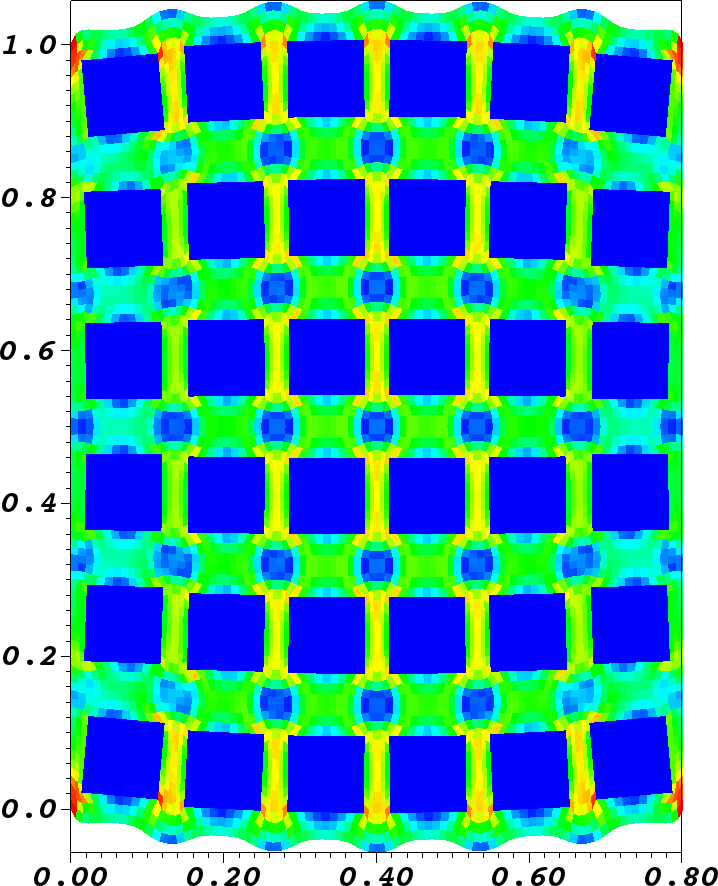
\includegraphics[width=\textwidth]{figures/MG/ElasticityCompressTrim}
    %\caption{Initial solution.}\label{fig:elast-initial}
  \end{subfigure} ~
  \begin{subfigure}[b]{0.18\textwidth}
    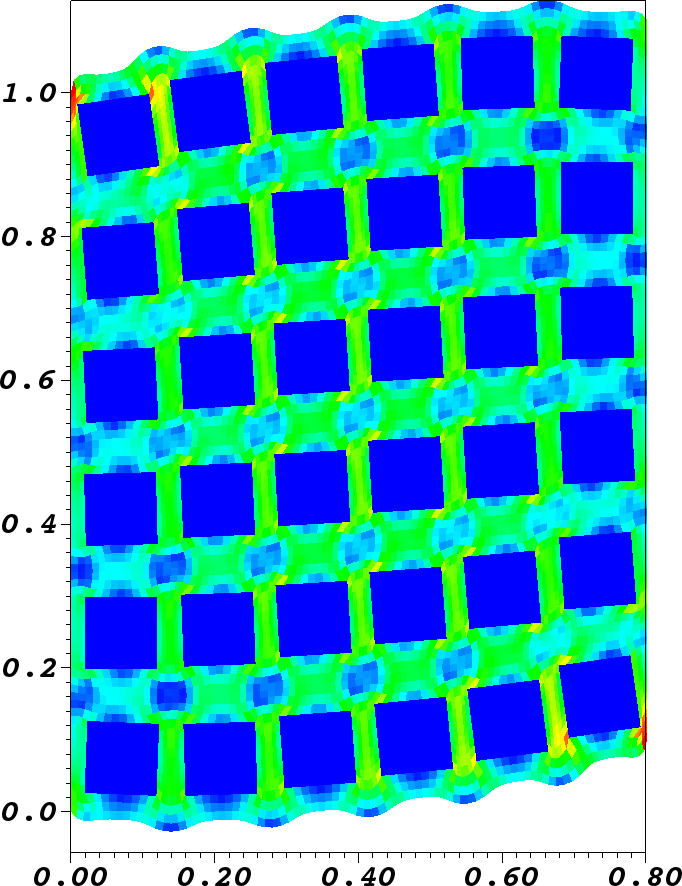
\includegraphics[width=\textwidth]{figures/MG/ElasticityCompressShearTrim}
    %\caption{Increment.}\label{fig:elast-increment}
  \end{subfigure} ~
  \begin{subfigure}[b]{0.28\textwidth}
    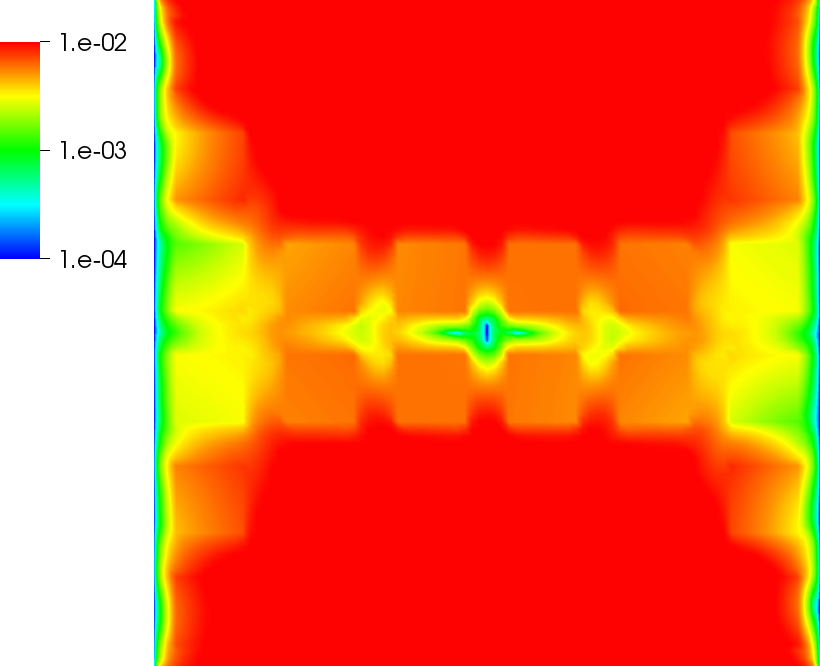
\includegraphics[width=\textwidth]{figures/MG/ElasticityCompressErrorNoTauTrim}
    %\caption{Smoothed error without $\tau$.}\label{fig:elast-error-notau}
  \end{subfigure} ~
  \begin{subfigure}[b]{0.28\textwidth}
    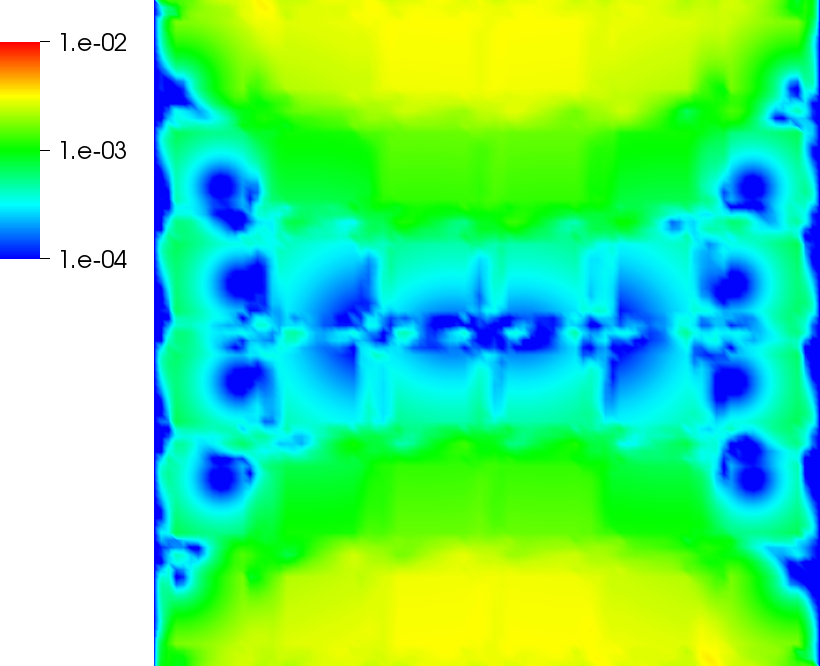
\includegraphics[width=\textwidth]{figures/MG/ElasticityCompressErrorTauTrim}
    %\caption{Smoothed error with $\tau$.}\label{fig:elast-error-tau}
  \end{subfigure}
  \begin{itemize}
  \item Plane strain elasticity, $E=1000,\nu=0.4$ inclusions in $E=1,\nu=0.2$ material, coarsen by $3^2$.
  \item Solve initial problem everywhere and compute $\tau_h^H = A^H \hat I_h^H u^h - I_h^H A^h u^h$
  \item Change boundary conditions and solve FAS coarse problem
    \begin{equation*}
      N^H \acute u^H = \underbrace{I_h^H \acute f^h}_{\acute f^H} + \underbrace{N^H \hat I_h^H \tilde u^h - I_h^H N^h \tilde u^h}_{\tau_h^H}
    \end{equation*}
  \item Prolong, post-smooth, compute error $e^h = \acute u^h - (N^h)^{-1} \acute f^h$
  \item<2> \alert{Coarse grid \emph{with $\tau$} is nearly $10\times$ better accuracy}
  \end{itemize}
  % \caption{Plane strain elasticity, $E=1000,\nu=0.4$ inclusions in $E=1,\nu=0.2$ material.  2-level multigrid with coarsening factor of $3^2$.
  %   Panes (a) and (b) show the deformed body colored by strain.
  %   The initial problem of compression by 0.2 from the right is solved (a) and $\tau = A^H \hat I_h^H u^h - I_h^H A^h u^h$ is computed.
  %   Then a shear increment of 0.1 in the $y$ direction is added to the boundary condition, and the coarse-level problem is resolved, interpolated to the fine-grid, and a post-smoother is applied.
  %   When the coarse problem is solved without a $\tau$ correction (c), the displacement error is nearly $10\times$ larger than when $\tau$ is included in the right hand side of the coarse problem (d).
  % }\label{fig:tau-valid}
  % ./ex49 -mx 90 -my 90 -da_refine_x 3 -da_refine_y 3 -elas_ksp_converged_reason -elas_ksp_rtol 1e-8 -no_view -c_str 3 -sponge_E0 1 -sponge_E1 1e3 -sponge_nu0 0.4 -sponge_nu1 0.2 -sponge_t 3 -sponge_w 9 -u_o vtk:ex49_sol.vts -use_nonsymbc -elas_pc_type mg -elas_pc_mg_levels 2 -elas_pc_mg_galerkin -tau1_o vtk:ex49_tau1.vts -tau2_o vtk:ex49_tau2.vts -taudiff_o vtk:ex49_taudiff.vts -u2_o vtk:ex49_sol2.vts -u2c_o vtk:ex49_sol2c.vts -u3_o vtk:ex49_sol3.vts -u4_o vtk:ex49_sol4.vts -u2err_o vtk:ex49_sol2err.vts -u3err_o vtk:ex49_sol3err.vts -u3c_o vtk:ex49_sol3c.vts -tau3_o vtk:ex49_tau3.vts
\end{figure}
\end{frame}

\begin{frame}{Low communication MG}
  \begin{columns}
    \begin{column}{0.55\textwidth}
      \begin{itemize}
      \item {\color{red} red arrows} can be removed by $\tau$-FAS with overlap
      \item {\color{blue} blue arrows} can also be removed, but then
        algebraic convergence stalls when discretization error is
        reached
      \item no simple way to check that discretization error is obtained
      \item if fine grid state is not stored, use compatible relaxation to complete prolongation $P$
      \item ``Segmental refinement'' by Achi Brandt (1977)
      \item 2-process case by Brandt and Diskin (1994)
      \end{itemize}
    \end{column}
    \begin{column}{0.45\textwidth}
      \vspace{-2em}
      \includegraphics[width=\textwidth]{figures/MG/LowCommunication}
    \end{column}
  \end{columns}
\end{frame}


\begin{frame}[fragile]{Multiscale compression and recovery using $\tau$ form}
   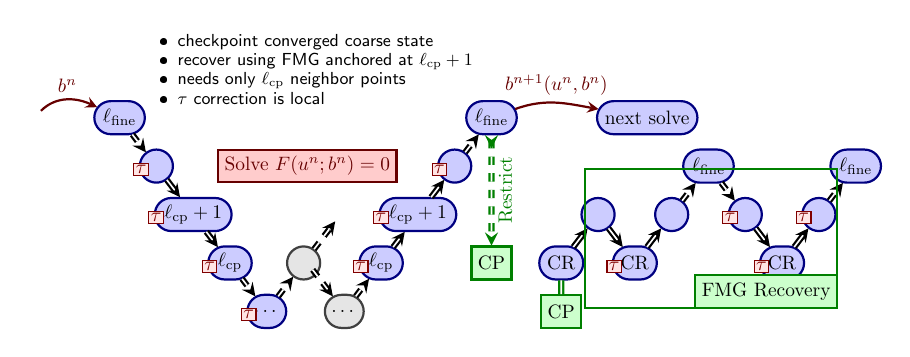
\begin{tikzpicture}
    [scale=0.7,every node/.style={scale=0.7},
    >=stealth,
    restrict/.style={thick,double},
    prolong/.style={thick,double},
    cprestrict/.style={green!50!black,thick,double,dashed},
    control/.style={rectangle,red!40!black,draw=red!40!black,thick},
    mglevel/.style={rounded rectangle,draw=blue!50!black,fill=blue!20,thick,minimum size=6mm},
    checkpoint/.style={rectangle,draw=green!50!black,fill=green!20,thick,minimum size=6mm},
    mglevelhide/.style={rounded rectangle,draw=gray!50!black,fill=gray!20,thick,minimum size=6mm},
    tau/.style={text=red!50!black,draw=red!50!black,fill=red!10,inner sep=1pt},
    crelax/.style={text=green!50!black,fill=green!10,inner sep=0pt}
    ]
    \begin{scope}
      \newcommand\mgdx{1.9em}
      \newcommand\mgdy{2.5em}
      \newcommand\mgloc[4]{(#1 + #4*\mgdx*#3,#2 + \mgdy*#3)}
      \node[mglevel] (fine0) at \mgloc{0}{0}{4}{-1} {\mglevelfine};
      \node[mglevel] (finem1down0) at \mgloc{0}{0}{3}{-1} {};
      \node[mglevel] (cp1down0) at \mgloc{0}{0}{2}{-1} {$\mglevelcp+1$};
      \node[mglevel] (cpdown0) at \mgloc{0}{0}{1}{-1} {\mglevelcp};
      \node[mglevel] (coarser0) at \mgloc{0}{0}{0}{0} {\ldots};

      \node[mglevelhide] (cpup0) at \mgloc{0}{0}{1}{1} {};
      \node (cp1up0) at \mgloc{0}{0}{2}{1} {};

      \node (cpdown1) at \mgloc{4em}{0}{1}{-1} {};
      \node[mglevelhide] (coarser1) at \mgloc{4em}{0}{0}{1} {\ldots};
      \node[mglevel] (cpup1) at \mgloc{4em}{0}{1}{1} {\mglevelcp};
      \node[mglevel] (cp1up1) at \mgloc{4em}{0}{2}{1} {$\mglevelcp+1$};
      \node[mglevel] (finem1up1) at \mgloc{4em}{0}{3}{1} {};
      \node[mglevel] (fine1) at \mgloc{4em}{0}{4}{1} {\mglevelfine};

      \draw[->,restrict,dashed] (fine0) -- (finem1down0);
      \draw[->,restrict] (finem1down0) -- (cp1down0);
      \draw[->,restrict] (cp1down0) -- (cpdown0);
      \draw[->,restrict,dashed] (cpdown0) -- (coarser0);
      \draw[->,prolong,dashed] (coarser0) -- (cpup0);
      \draw[->,prolong,dashed] (cpup0) -- (cp1up0);

      \draw[->,restrict,dashed] (cpdown1) -- (coarser1);
      \draw[->,prolong,dashed] (coarser1) -- (cpup1);
      \draw[->,prolong] (cpup1) -- (cp1up1);
      \draw[->,prolong] (cp1up1) -- (finem1up1);
      \draw[->,prolong,dashed] (finem1up1) -- (fine1);

      \node[checkpoint] at (4em + \mgdx*4,\mgdy) (cp) {CP};
      \draw[>->,cprestrict] (fine1) -- node[below,sloped] {Restrict} (cp);

      \node[left=\mgdx of fine0] (bnanchor) {};
      \node[control,fill=red!20] at (1.1*\mgdx,3*\mgdy) {Solve $F(u^n;b^n) = 0$};
      \node[mglevel,right=of fine1] (finedt) {next solve};
      \draw[->, >=stealth, control] (fine1) to[out=20,in=170] node[above] {$b^{n+1}(u^n,b^n)$} (finedt);
      \draw[->, >=stealth, control] (bnanchor) to[out=45,in=155] node[above] {$b^n$} (fine0);

      % Recovery process
      \begin{scope}[xshift=8*\mgdx]
        \node[checkpoint] (rcp) at \mgloc{0}{0}{0}{0} {CP};
        \node[mglevel] (r0a) at \mgloc{0}{\mgdy}{0}{0} {CR};
        \node[mglevel] (r1a) at \mgloc{0}{\mgdy}{1}{1} {};
        \node[mglevel] (r0b) at \mgloc{2*\mgdx}{\mgdy}{0}{0} {CR};
        \node[mglevel] (r1b) at \mgloc{2*\mgdx}{\mgdy}{1}{1} {};
        \node[mglevel] (r2b) at \mgloc{2*\mgdx}{\mgdy}{2}{1} {\mglevelfine};
        \node[mglevel] (r1c) at \mgloc{6*\mgdx}{\mgdy}{1}{-1} {};
        \node[mglevel] (r0d) at \mgloc{6*\mgdx}{\mgdy}{0}{0} {CR};
        \node[mglevel] (r1d) at \mgloc{6*\mgdx}{\mgdy}{1}{1} {};
        \node[mglevel] (r2d) at \mgloc{6*\mgdx}{\mgdy}{2}{1} {\mglevelfine};

        \draw[-,prolong,green!50!black] (rcp) -- (r0a);
        \draw[->,prolong] (r0a) -- (r1a);
        \draw[->,restrict] (r1a) -- (r0b);
        \draw[->,restrict] (r0b) -- (r1b);
        \draw[->,restrict,dashed] (r1b) -- (r2b);
        \draw[->,restrict,dashed] (r2b) -- (r1c);
        \draw[->,restrict] (r1c) -- (r0d);
        \draw[->,restrict] (r0d) -- (r1d);
        \draw[->,restrict,dashed] (r1d) -- (r2d);

        \foreach \smooth in {finem1down0, cp1down0, cpdown0, coarser0,
          cpup1, cp1up1, finem1up1,
          r0b,r1c,r0d,r1d} {
          \node[above left=-5pt of \smooth.west,tau] {$\tau$};
        }
        \node[rectangle,fill=none,draw=green!50!black,thick,fit=(rcp)(r2d)] (recoverbox) {};
        \node[rectangle,draw=green!50!black,fill=green!20,thick,minimum size=6mm,above={0cm of recoverbox.south east},anchor=south east] (recover) {FMG Recovery};
      \end{scope}
      \node (notation) at (\mgdx,5*\mgdy) {
        \begin{minipage}{18em}\small\sf
          \begin{itemize}\addtolength{\itemsep}{-5pt}
          \item checkpoint converged coarse state
          \item recover using FMG anchored at $\mglevelcp+1$
          \item needs only $\mglevelcp$ neighbor points
          \item $\tau$ correction is local
          \end{itemize}
        \end{minipage}
      };
    \end{scope}
  \end{tikzpicture}
  \begin{itemize}
  \item Normal multigrid cycles visit all levels moving from $n \to n+1$
  \item FMG recovery only accesses levels finer than $\ell_{CP}$
  \item Only failed processes and neighbors participate in recovery
  \item Lightweight checkpointing for transient adjoint computation
  \item Postprocessing applications, e.g., in-situ visualization at high temporal resolution in part of the domain
  \end{itemize}
\end{frame}

\begin{frame}\LARGE
  \begin{itemize}
  \item Maximize science per Watt
  \item Huge scope remains at problem formulation
  \item Raise level of abstraction at which a problem is formally specified
  \item Algorithmic optimality is crucial
  \item Improve matrix-free abstractions, robustness, diagnostics
  \item Better language/library support for aggregating
  \end{itemize}
\end{frame}

\end{document}
